\subsection{Experiments 4--7: Temporal Forecasting}

% ---- Experiment 4 - GlobalPlasticsProduction

Producing business-as-usual projections from historical data is a fundamental task in environmental data analysis. In this study, we design four experiments to evaluate the performance of various forecasting methods across datasets with different characteristics.

In Experiment 4, we apply forecasting models to the \texttt{GlobalPlasticsProduction} dataset. This dataset contains 59 samples, making it relatively large for time series analysis; therefore, machine learning models are expected to perform well. This experiment serves as a benchmark for evaluating model performance on larger datasets. Additionally, we tune hyperparameters using both grid search and random search methods, and compare their runtime and performance.

\begin{figure}[H]
	\centering
	\subfloat[Theil-Sen regression.]{
		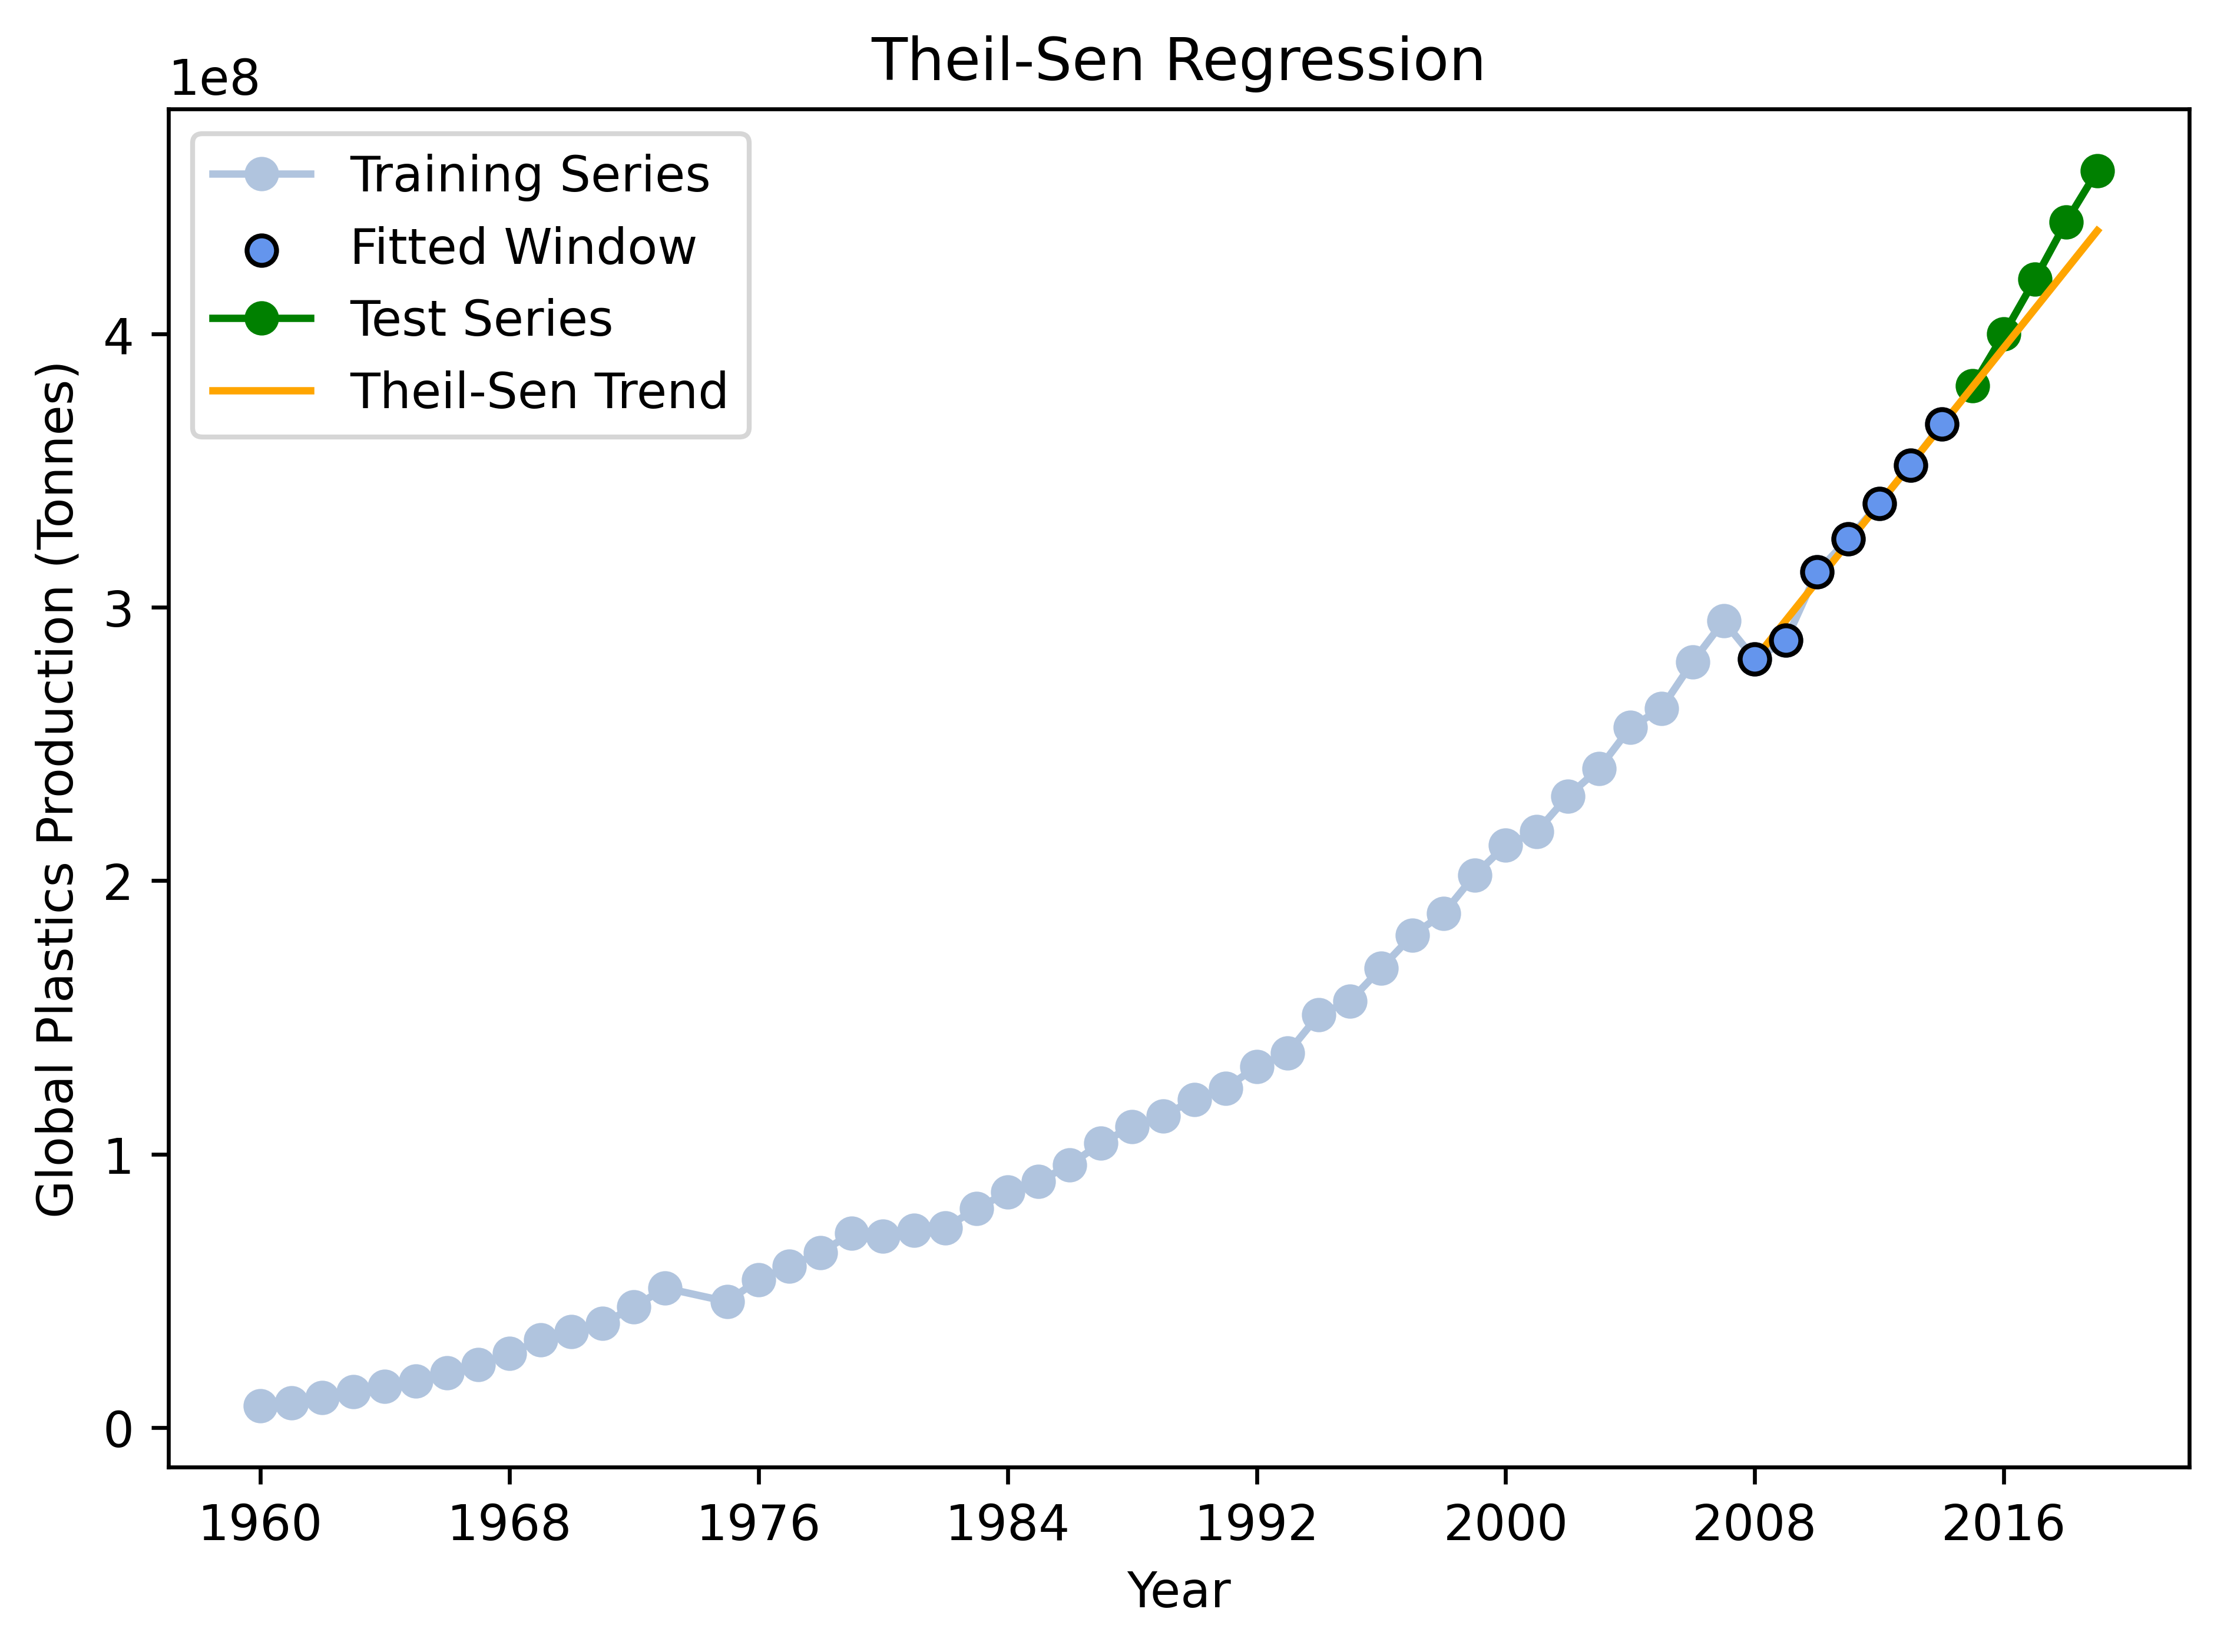
\includegraphics[width=0.45\textwidth]{figures/global_forecasting_theil_sen_regression.png}
	}
	\hfill
	\subfloat[Ridge regression.]{
		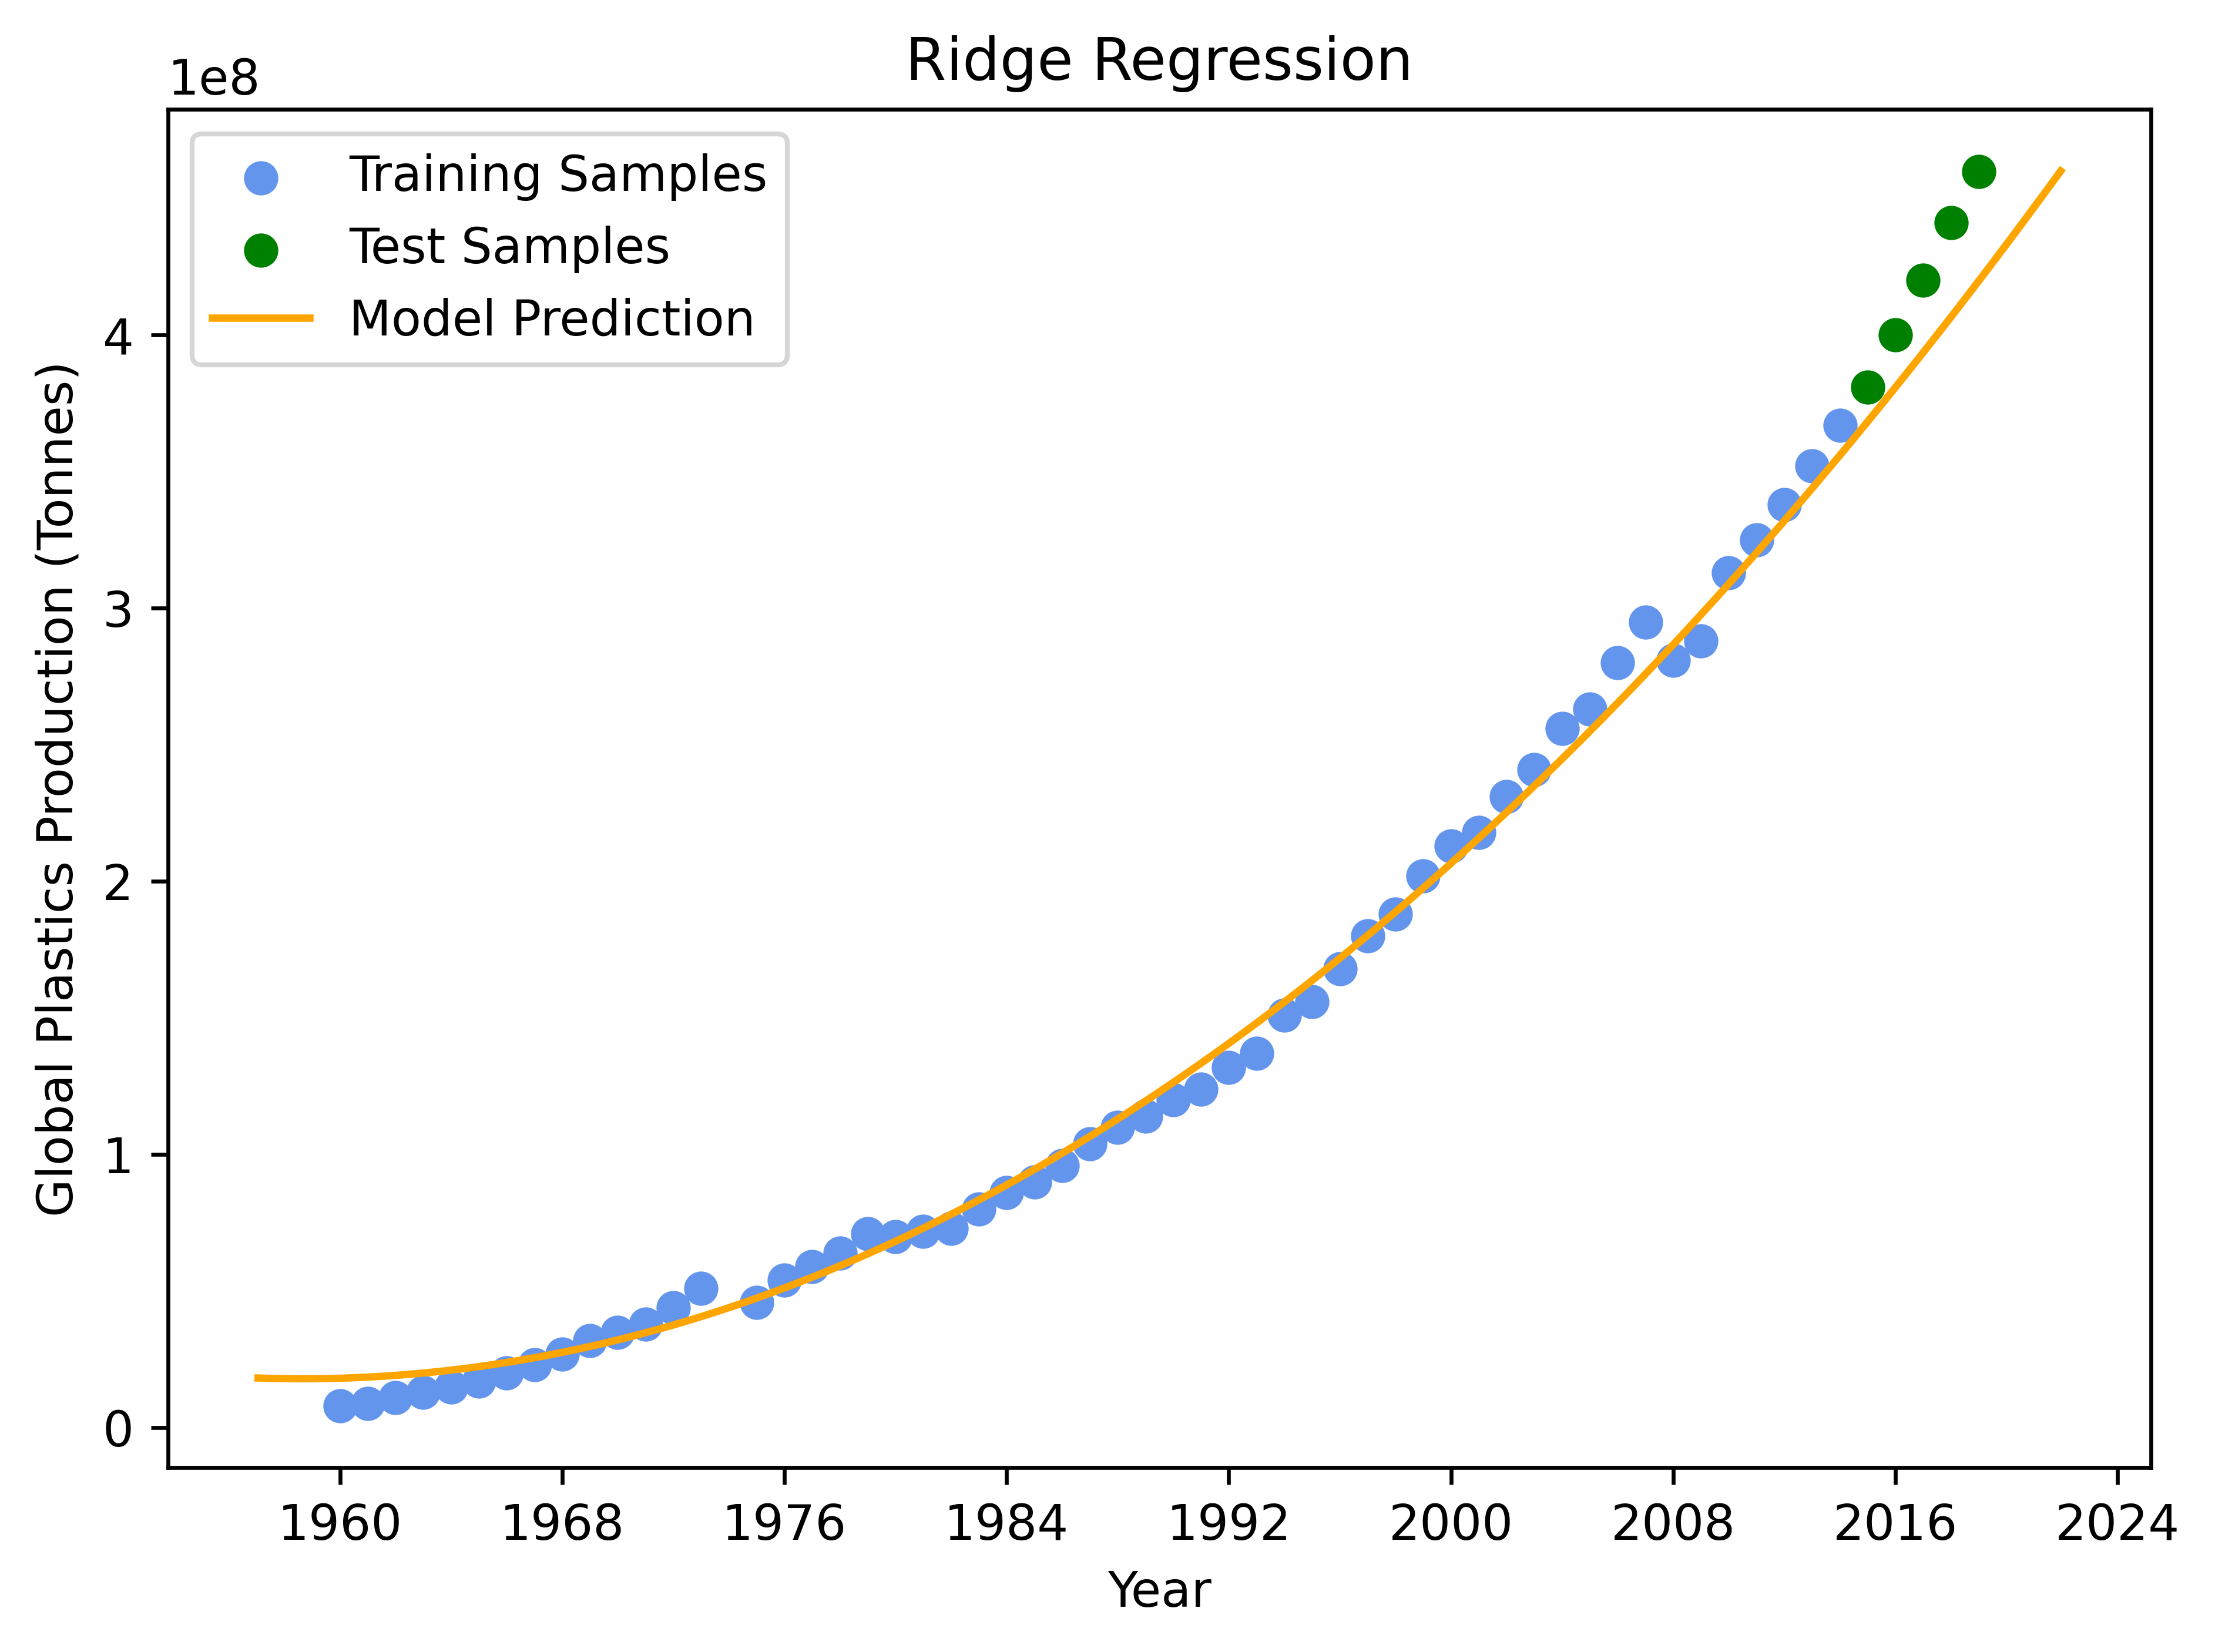
\includegraphics[width=0.45\textwidth]{figures/global_forecasting_ridge_regression.png}
	}

	\vspace{0.5cm}

	\subfloat[Gaussian process regression.]{
		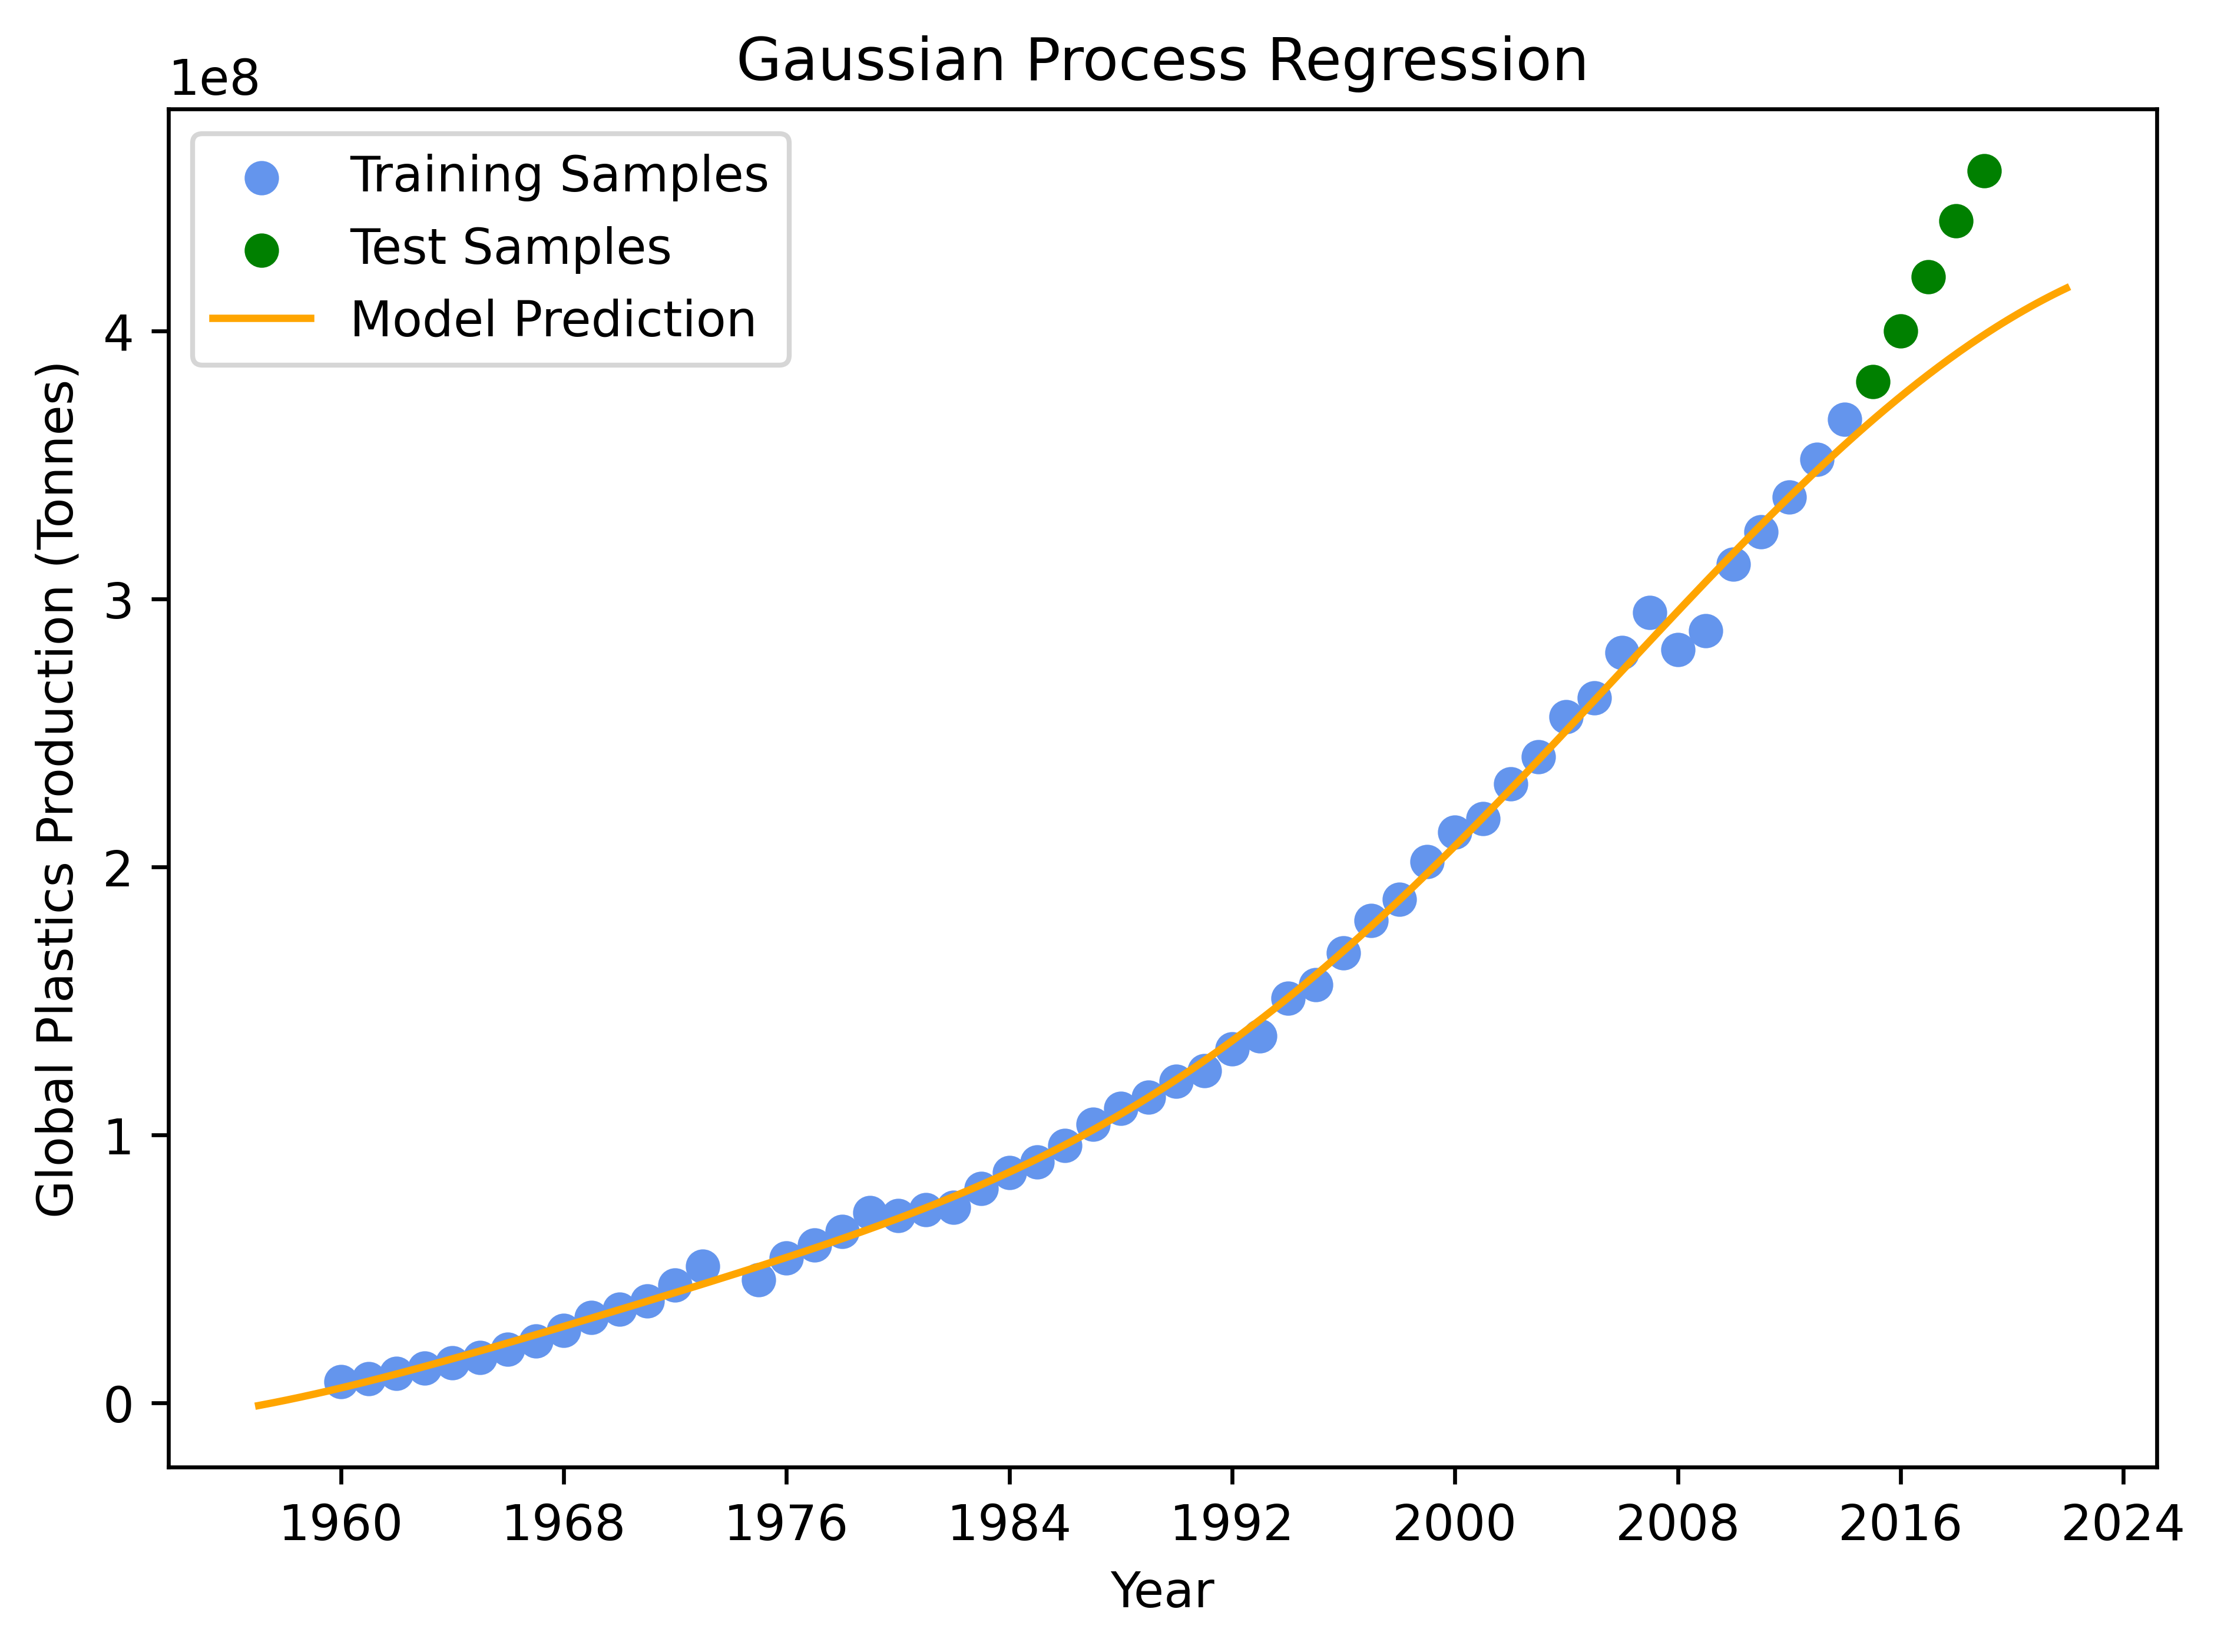
\includegraphics[width=0.45\textwidth]{figures/global_forecasting_gpr.png}
	}
	\subfloat[Support vector regression.]{
		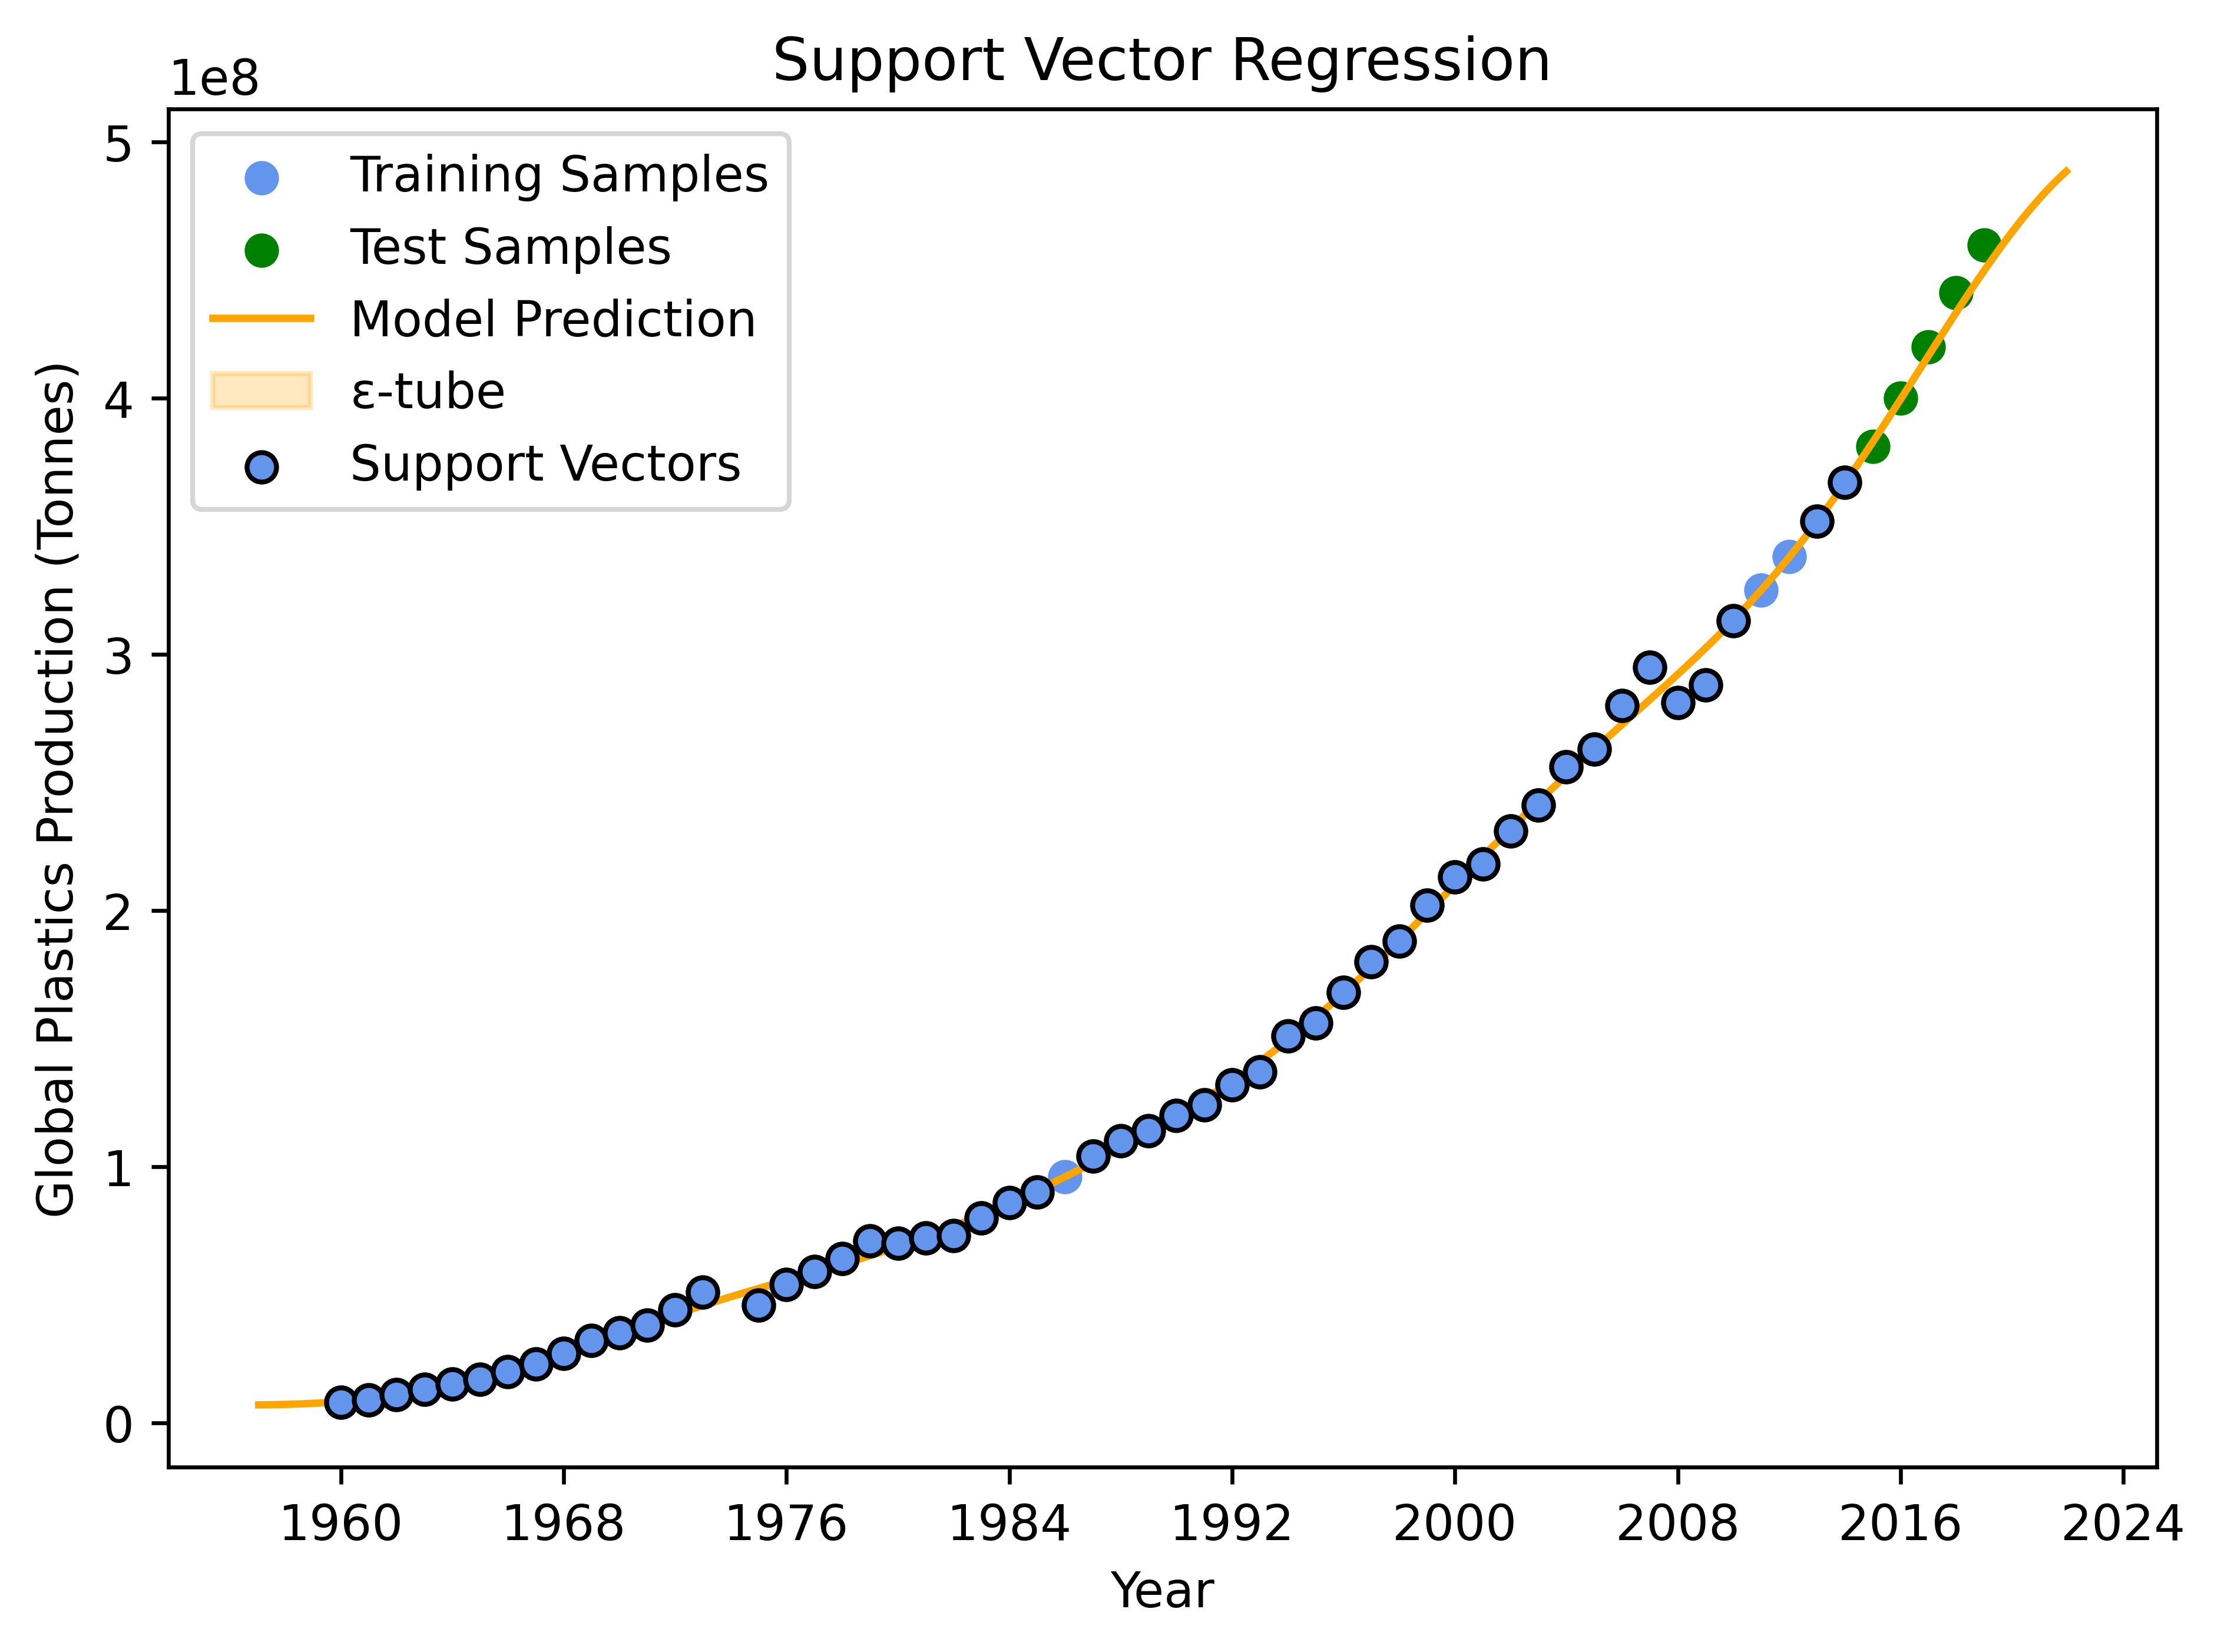
\includegraphics[width=0.45\textwidth]{figures/global_forecasting_svr.png}
	}

	\caption{Forecasts of global plastic production produced by four representative regression models.}
	\label{fig:global_forecasting_plots}
\end{figure}

\begin{table}[!ht]
	\centering
	\caption{
		\centering Temporal forecasting performance for global plastic production using grid-search tuning for tunable models. The \textsuperscript{*} marker denotes the SVR variant with \(\gamma\) tuning enabled.
	}
	\begin{tabular}{@{}lccccc@{}}
		\toprule
		\textbf{Experiment}                          & \textbf{MAE}                   & \textbf{RMSE}                  & $\mathbf{R^2}$     & \textbf{WAPE}       & \textbf{MAPE}       \\
		\midrule
		Naive Persistence                            & \(5.338 \times 10^7\)          & \(6.031 \times 10^7\)          & -3.615             & 12.70\%             & 12.31\%             \\
		Drift Baseline                               & \(3.344 \times 10^7\)          & \(3.830 \times 10^7\)          & -0.861             & 7.95\%              & 7.69\%              \\
		Exponential Smoothing                        & \(1.792 \times 10^7\)          & \(2.103 \times 10^7\)          & 0.439              & 4.26\%              & 4.10\%              \\
		Ridge Regression                             & \(3.261 \times 10^7\)          & \(3.421 \times 10^7\)          & -0.484             & 7.76\%              & 7.63\%              \\
		Gaussian Process Regression                  & \(3.722 \times 10^7\)          & \(4.086 \times 10^7\)          & -1.118             & 8.85\%              & 8.63\%              \\
		\textbf{Support Vector Regression}           & \(\mathbf{7.921 \times 10^6}\) & \(\mathbf{9.942 \times 10^6}\) & \(\mathbf{0.875}\) & \(\mathbf{1.88}\)\% & \(\mathbf{1.80}\)\% \\
		Support Vector Regression\textsuperscript{*} & \(2.590 \times 10^7\)          & \(2.806 \times 10^7\)          & 0.001              & 6.16\%              & 6.02\%              \\
		Theil-Sen Regression                         & \(1.111 \times 10^7\)          & \(1.365 \times 10^7\)          & 0.764              & 2.64\%              & 2.53\%              \\
		ARIMA Regression                             & \(2.103 \times 10^7\)          & \(2.477 \times 10^7\)          & 0.222              & 5.00\%              & 4.81\%              \\
		\hline
	\end{tabular}
	\label{tab:global_forecasting_grid_search_metric_table}
\end{table}

\begin{table}[!ht]
	\centering
	\caption{\centering Temporal forecasting performance for global plastic production using random-search tuning for tunable models. The \textsuperscript{*} marker denotes the SVR variant with \(\gamma\) tuning enabled.}
	\begin{tabular}{@{}lccccc@{}}
		\toprule
		\textbf{Experiment}                          & \textbf{MAE}                   & \textbf{RMSE}                  & $\mathbf{R^2}$     & \textbf{WAPE}       & \textbf{MAPE}       \\
		\midrule
		Naive Persistence                            & \(5.338 \times 10^7\)          & \(6.031 \times 10^7\)          & -3.615             & 12.70\%             & 12.31\%             \\
		Drift Baseline                               & \(3.344 \times 10^7\)          & \(3.830 \times 10^7\)          & -0.861             & 7.95\%              & 7.69\%              \\
		Exponential Smoothing                        & \(1.792 \times 10^7\)          & \(2.103 \times 10^7\)          & 0.439              & 4.26\%              & 4.10\%              \\
		Ridge Regression                             & \(2.657 \times 10^7\)          & \(2.834 \times 10^7\)          & -0.019             & 6.32\%              & 6.19\%              \\
		Gaussian Process Regression                  & \(3.722 \times 10^7\)          & \(4.086 \times 10^7\)          & -1.118             & 8.85\%              & 8.63\%              \\
		\textbf{Support Vector Regression}           & \(\mathbf{4.709 \times 10^6}\) & \(\mathbf{5.913 \times 10^6}\) & \(\mathbf{0.956}\) & \(\mathbf{1.12}\)\% & \(\mathbf{1.07}\)\% \\
		Support Vector Regression\textsuperscript{*} & \(2.503 \times 10^7\)          & \(2.727 \times 10^7\)          & 0.057              & 5.95\%              & 5.81\%              \\
		Theil-Sen Regression                         & \(1.111 \times 10^7\)          & \(1.365 \times 10^7\)          & 0.764              & 2.64\%              & 2.53\%              \\
		ARIMA Regression                             & \(2.103 \times 10^7\)          & \(2.477 \times 10^7\)          & 0.222              & 5.00\%              & 4.81\%              \\
		\hline
	\end{tabular}
	\label{tab:global_forecasting_random_search_metric_table}
\end{table}

% Table~\ref{tab:forecasting_results_grid_search} and Table~\ref{tab:forecasting_results_random_search} show that SVR achieved the best overall performance among all evaluated methods. In the random search tuning setting, SVR obtained the lowest MAE, RMSE, WAPE, and MAPE, and the highest \(R^2\) value. In the grid search tuning setting, SVR is also the best performing method, although it was slightly weaker than in the former setting. These results indicate that SVR was the most effective model for capturing the temporal trend in global plastic production. Figure~\ref{fig:global_forecasting_plots} visually confirms the superior performance of SVR, as its forecasted test values closely follow the actual test values, while the other methods show larger deviations.

Table~\ref{tab:global_forecasting_grid_search_metric_table} and Table~\ref{tab:global_forecasting_random_search_metric_table} indicate that SVR achieved the best overall performance among all evaluated methods. Under the random search tuning setting, SVR attained the lowest MAE, RMSE, WAPE, and MAPE, as well as the highest \(R^2\) value. Under the grid search setting, SVR also remained the top-performing method, although its performance was slightly inferior to that of the random search setting.

These results suggest that SVR is the most effective model for capturing the temporal trend in global plastic production. Figure~\ref{fig:global_forecasting_plots} further supports this conclusion, as the SVR forecasts closely follow the actual test values, whereas the other methods exhibit larger deviations.

\begin{table}[!ht]
	\centering
	\caption{
		\centering Hyperparameter tuning time for tunable global plastic production forecasting models under grid search and random search. The \textsuperscript{*} marker denotes the SVR variant with \(\gamma\) tuning enabled.
	}
	\begin{tabular}{@{}lcc@{}}
		\toprule
		\textbf{Experiment}                          & \textbf{Grid Search (ms)} & \textbf{Random Search (ms)} \\
		\midrule
		Ridge Regression                             & 6331.585                  & 2985.758                    \\
		Gaussian Process Regression                  & 158576.799                & 133046.250                  \\
		Support Vector Regression                    & 4150.489                  & 3186.485                    \\
		Support Vector Regression\textsuperscript{*} & 61600.061                 & 2771.060                    \\
		\hline
	\end{tabular}
	\label{tab:forecasting_tuning_time}
\end{table}

% Table~\ref{tab:forecasting_results_grid_search} and Table~\ref{tab:forecasting_results_random_search} also show that for all the tunable models, random search always has equal to better performance than grid search. Moreover, Table~\ref{tab:forecasting_tuning_time} suggests that random search is more efficient than grid search in terms of hyperparameter tuning time in this experiment settings. Therefore, in the following experiments, we will only report the results of random search tuning for the tunable models.

Table~\ref{tab:global_forecasting_grid_search_metric_table} and Table~\ref{tab:global_forecasting_random_search_metric_table} also show that, for all tunable models, random search consistently achieves performance that is equal to or better than that of grid search. Furthermore, Table~\ref{tab:forecasting_tuning_time} indicates that random search is more efficient in terms of hyperparameter tuning time under the experimental settings considered. Therefore, in the subsequent experiments, we report only the results obtained using random search for the tunable models.

% ---- Experiment 5 - YearPWG (Japan)

In Experiment 5, we evaluate the same forecasting models on the \texttt{YearPWG (Japan)} dataset. This series contains only 26 annual observations, so the hold-out set is small, and the model rankings should be interpreted cautiously.

\begin{figure}[H]
	\centering
	\subfloat[Arima regression.]{
		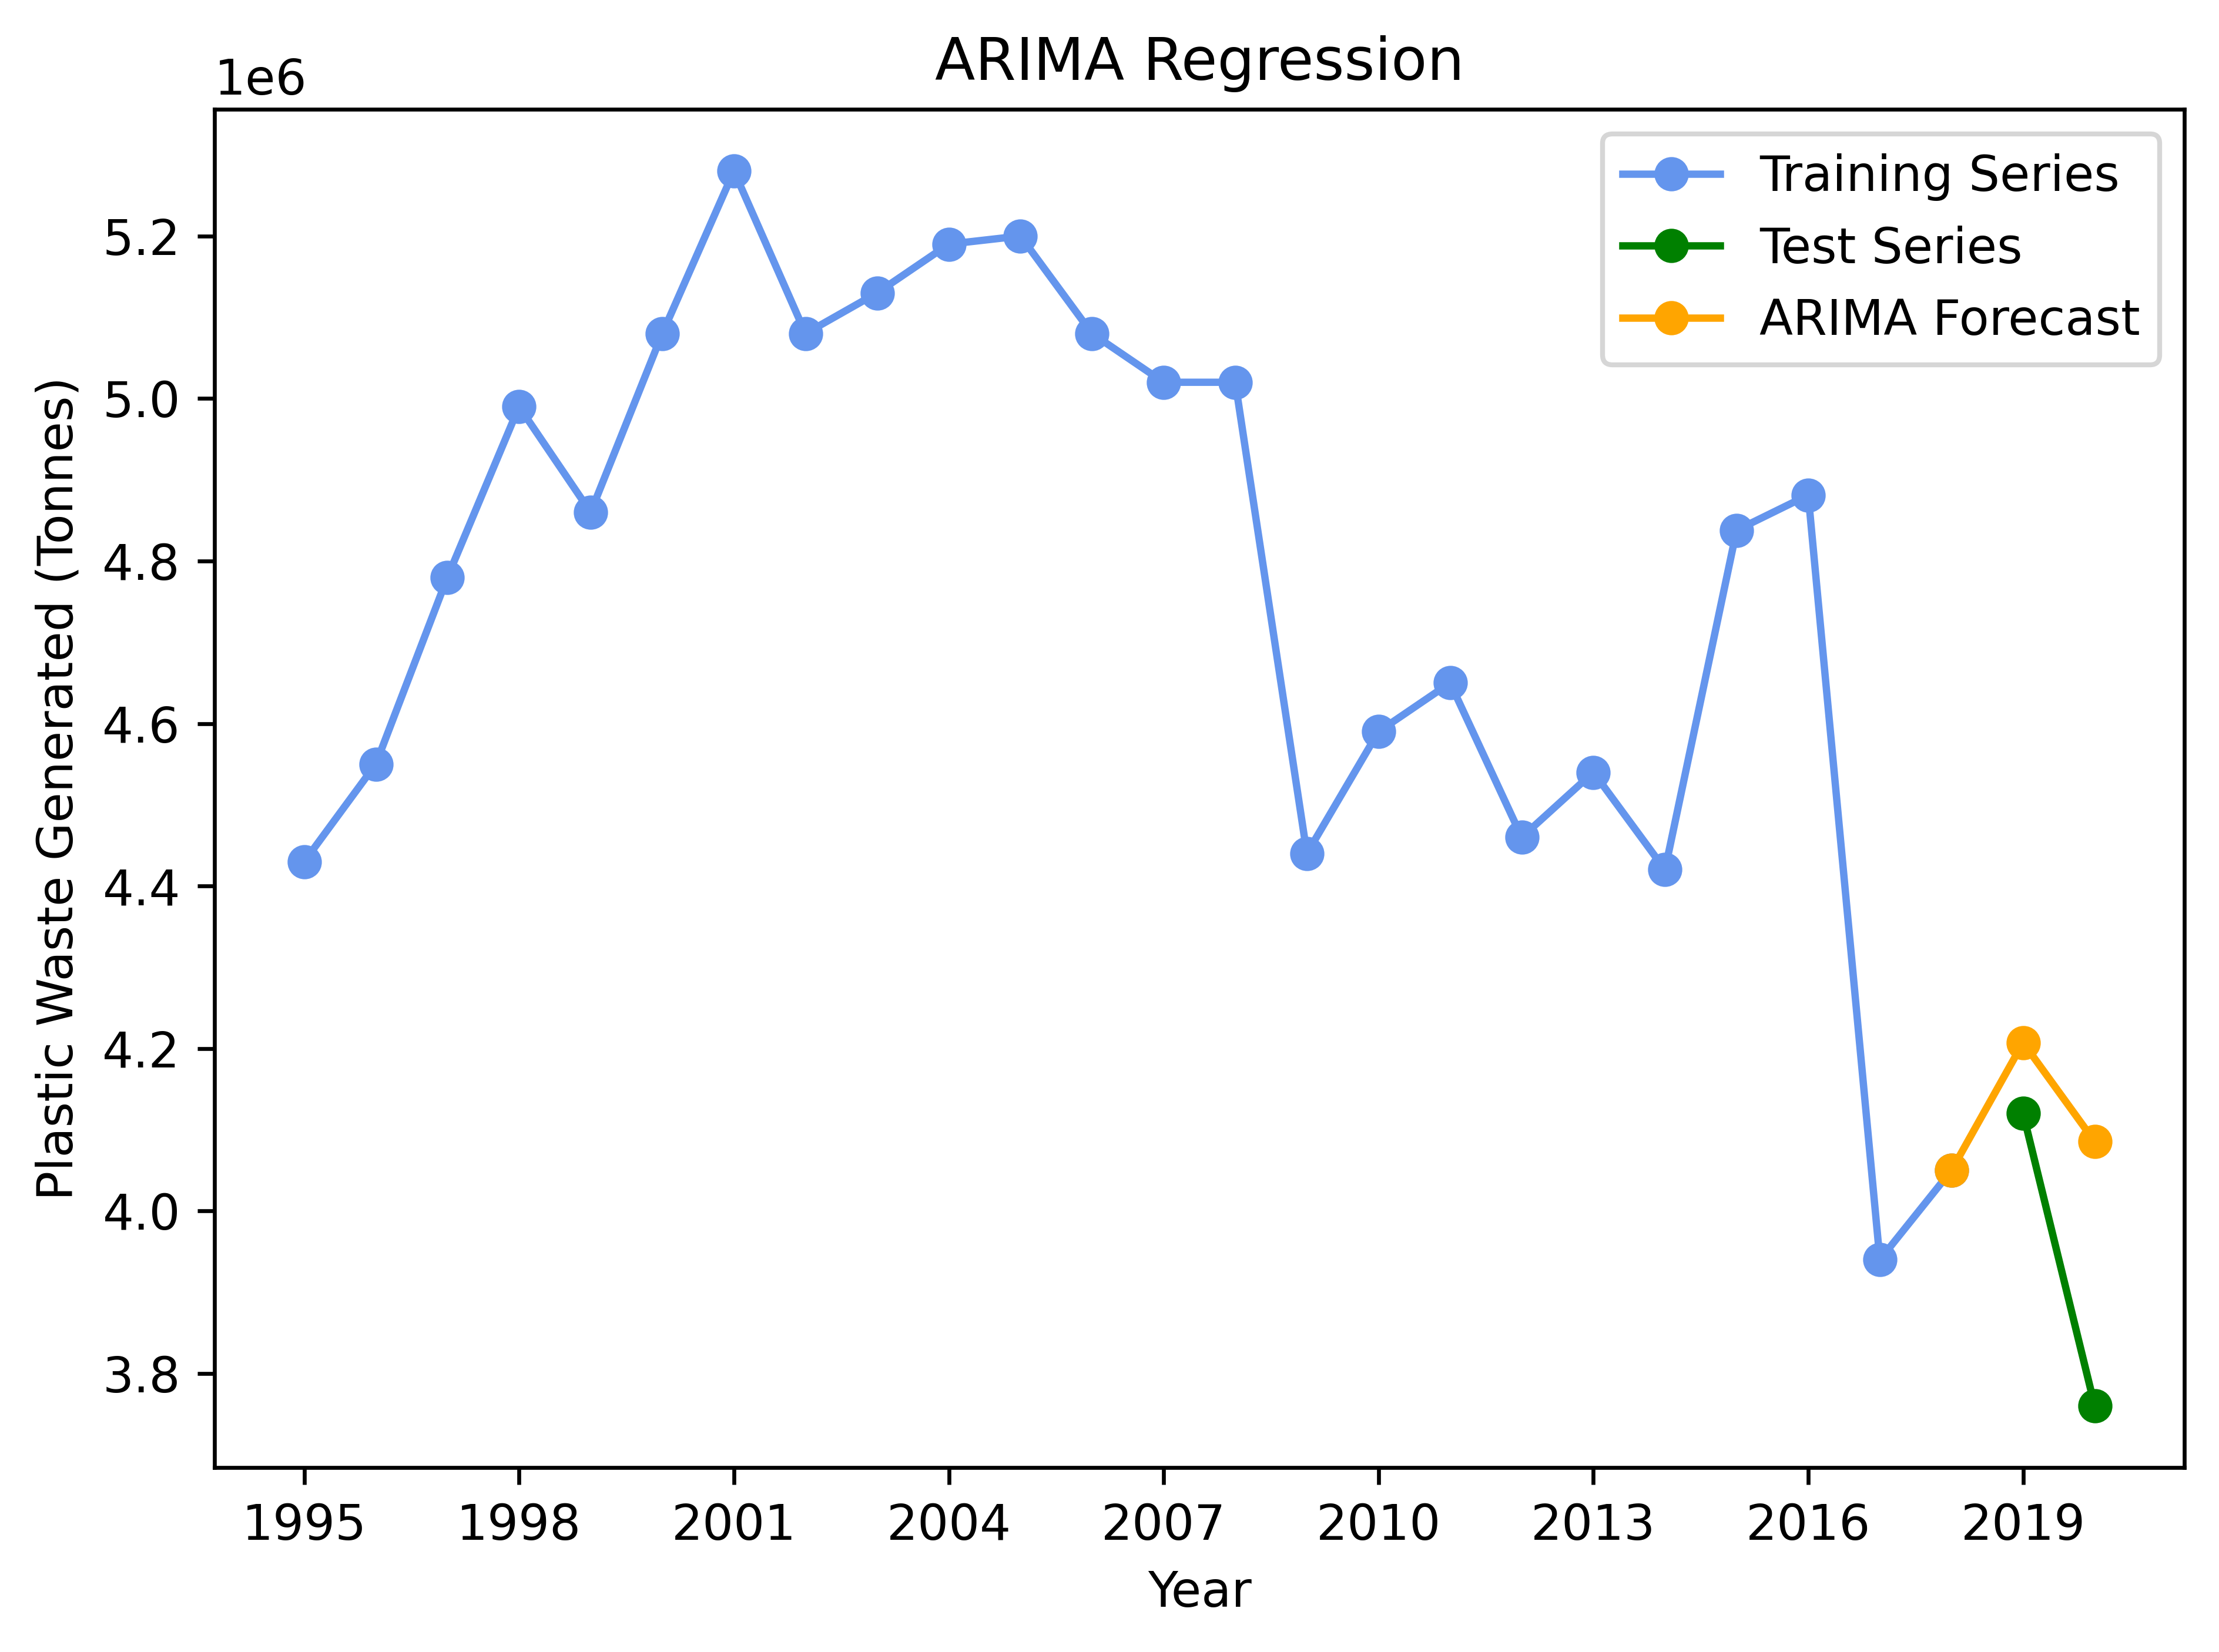
\includegraphics[width=0.45\textwidth]{figures/japan_pwg_forecasting_arima_regression.png}
	}
	\hfill
	\subfloat[Ridge regression.]{
		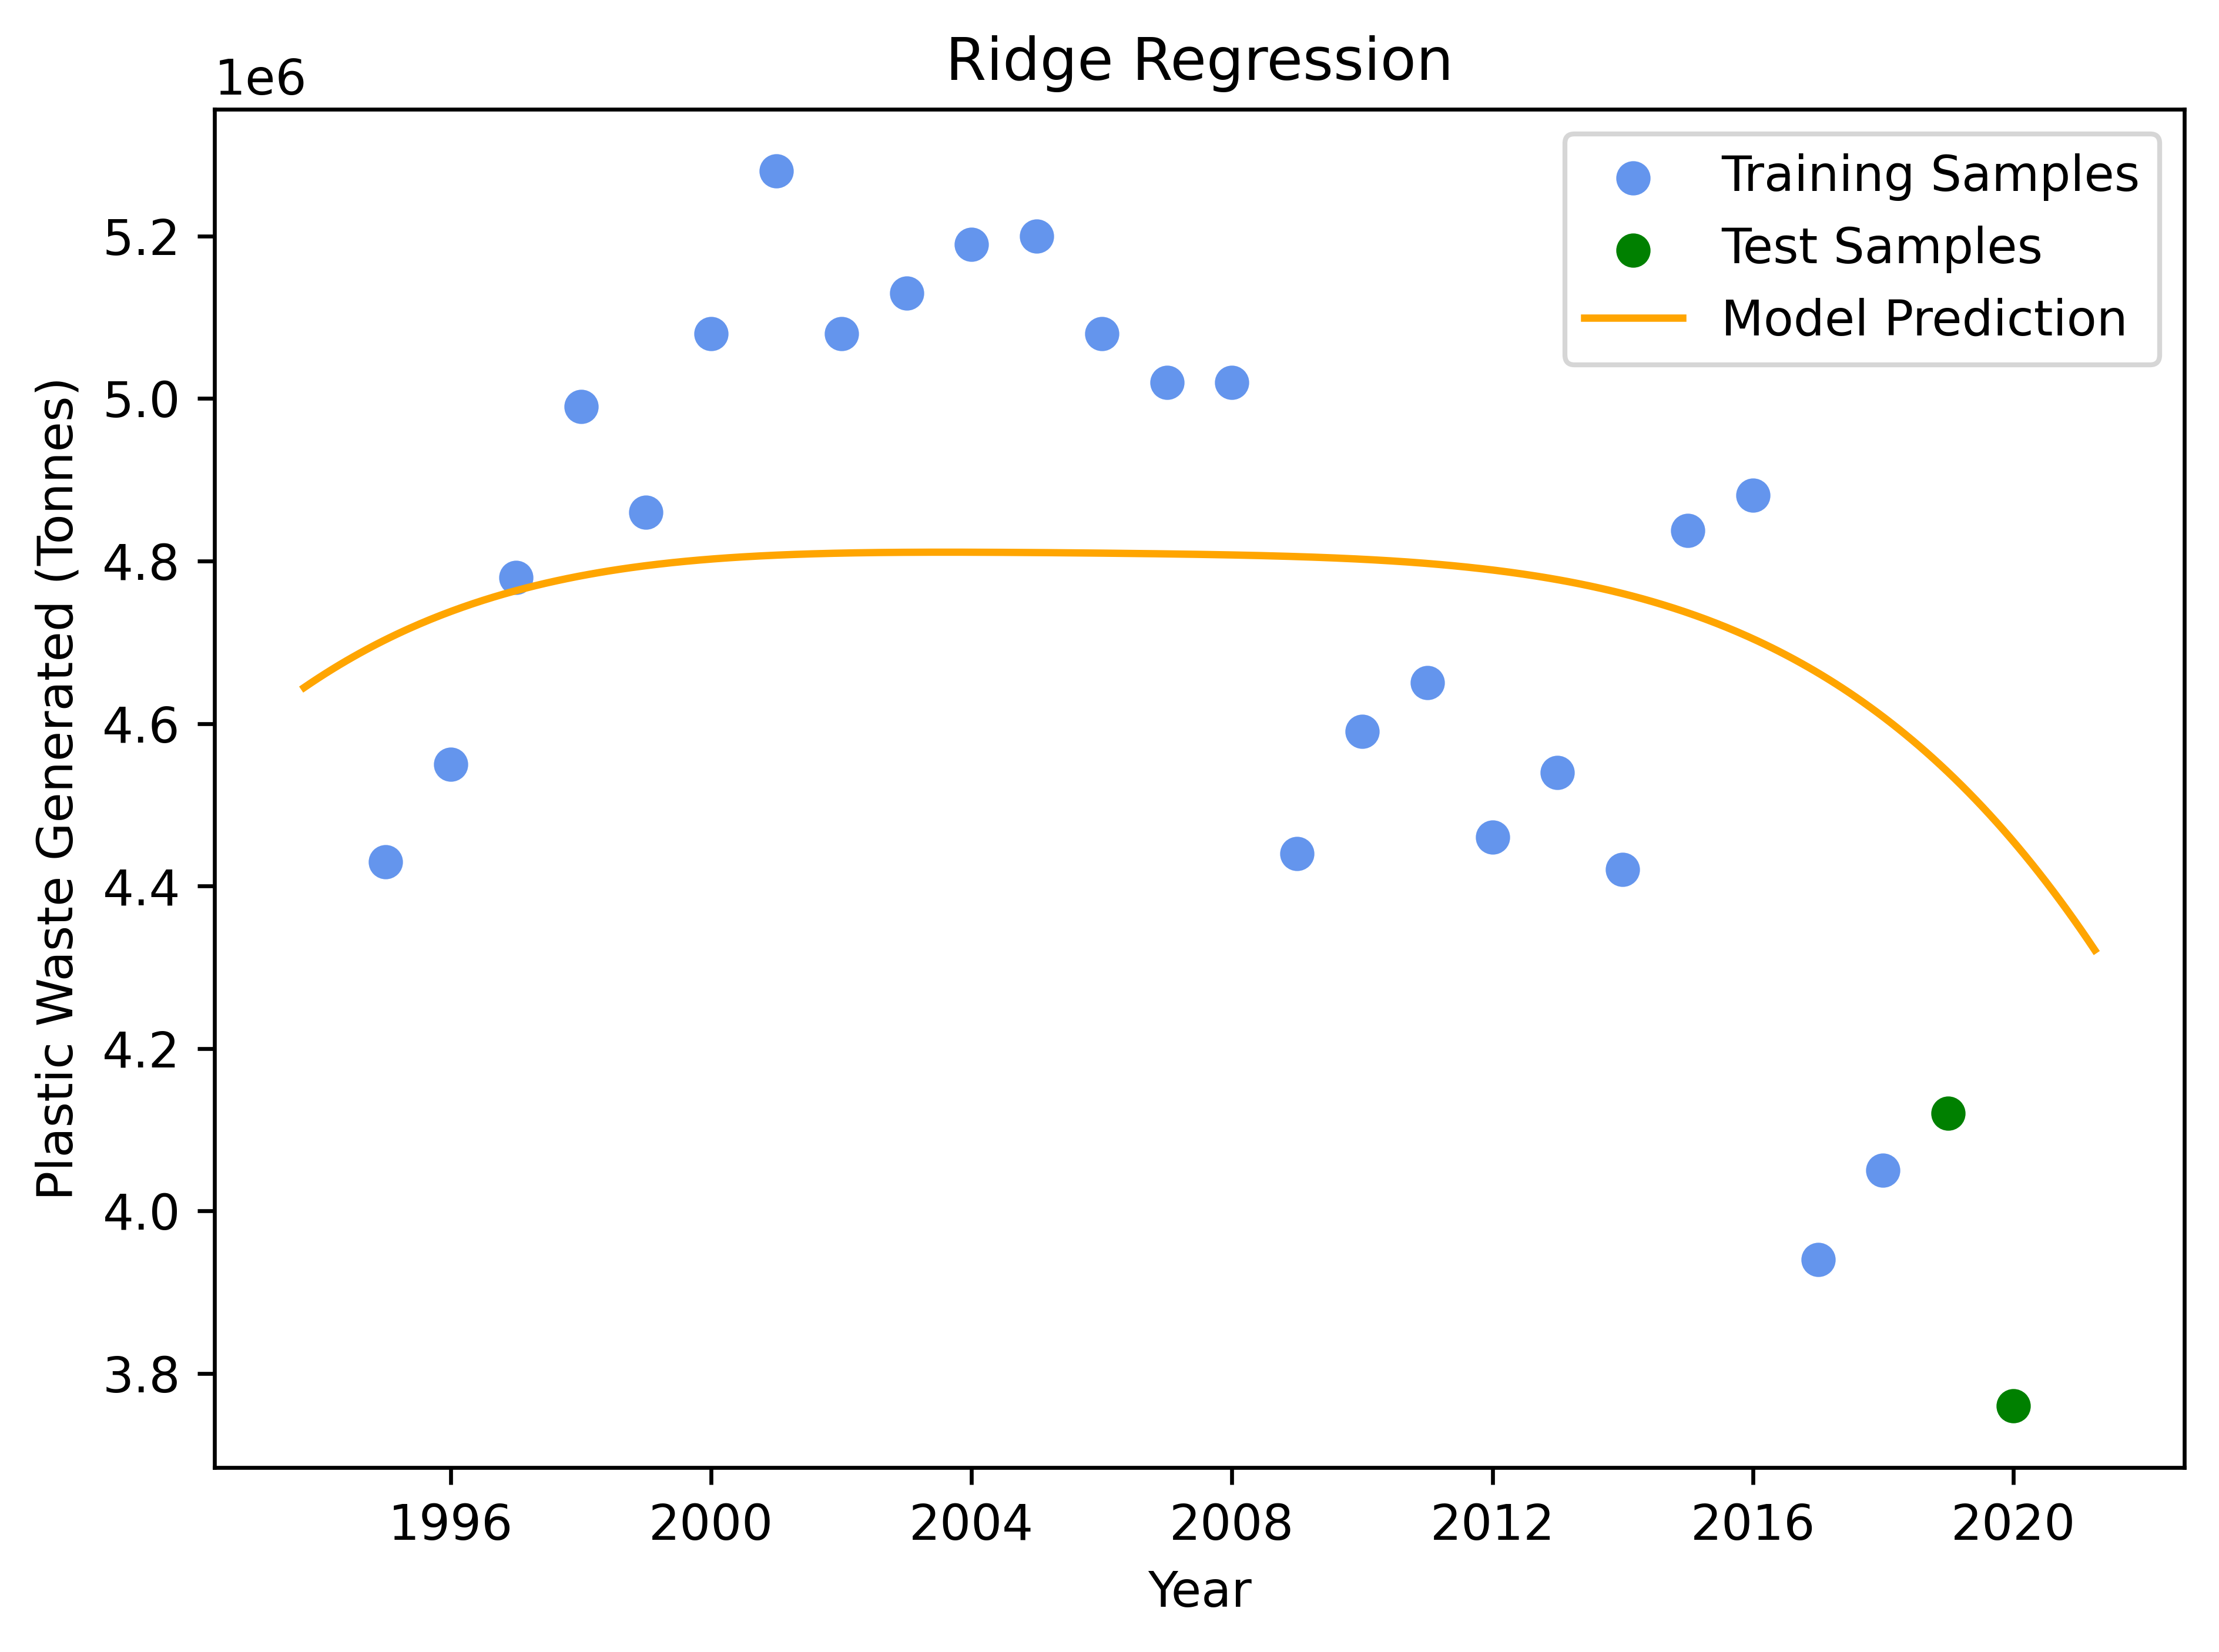
\includegraphics[width=0.45\textwidth]{figures/japan_pwg_forecasting_ridge_regression.png}
	}

	\vspace{0.5cm}

	\subfloat[Gaussian process regression.]{
		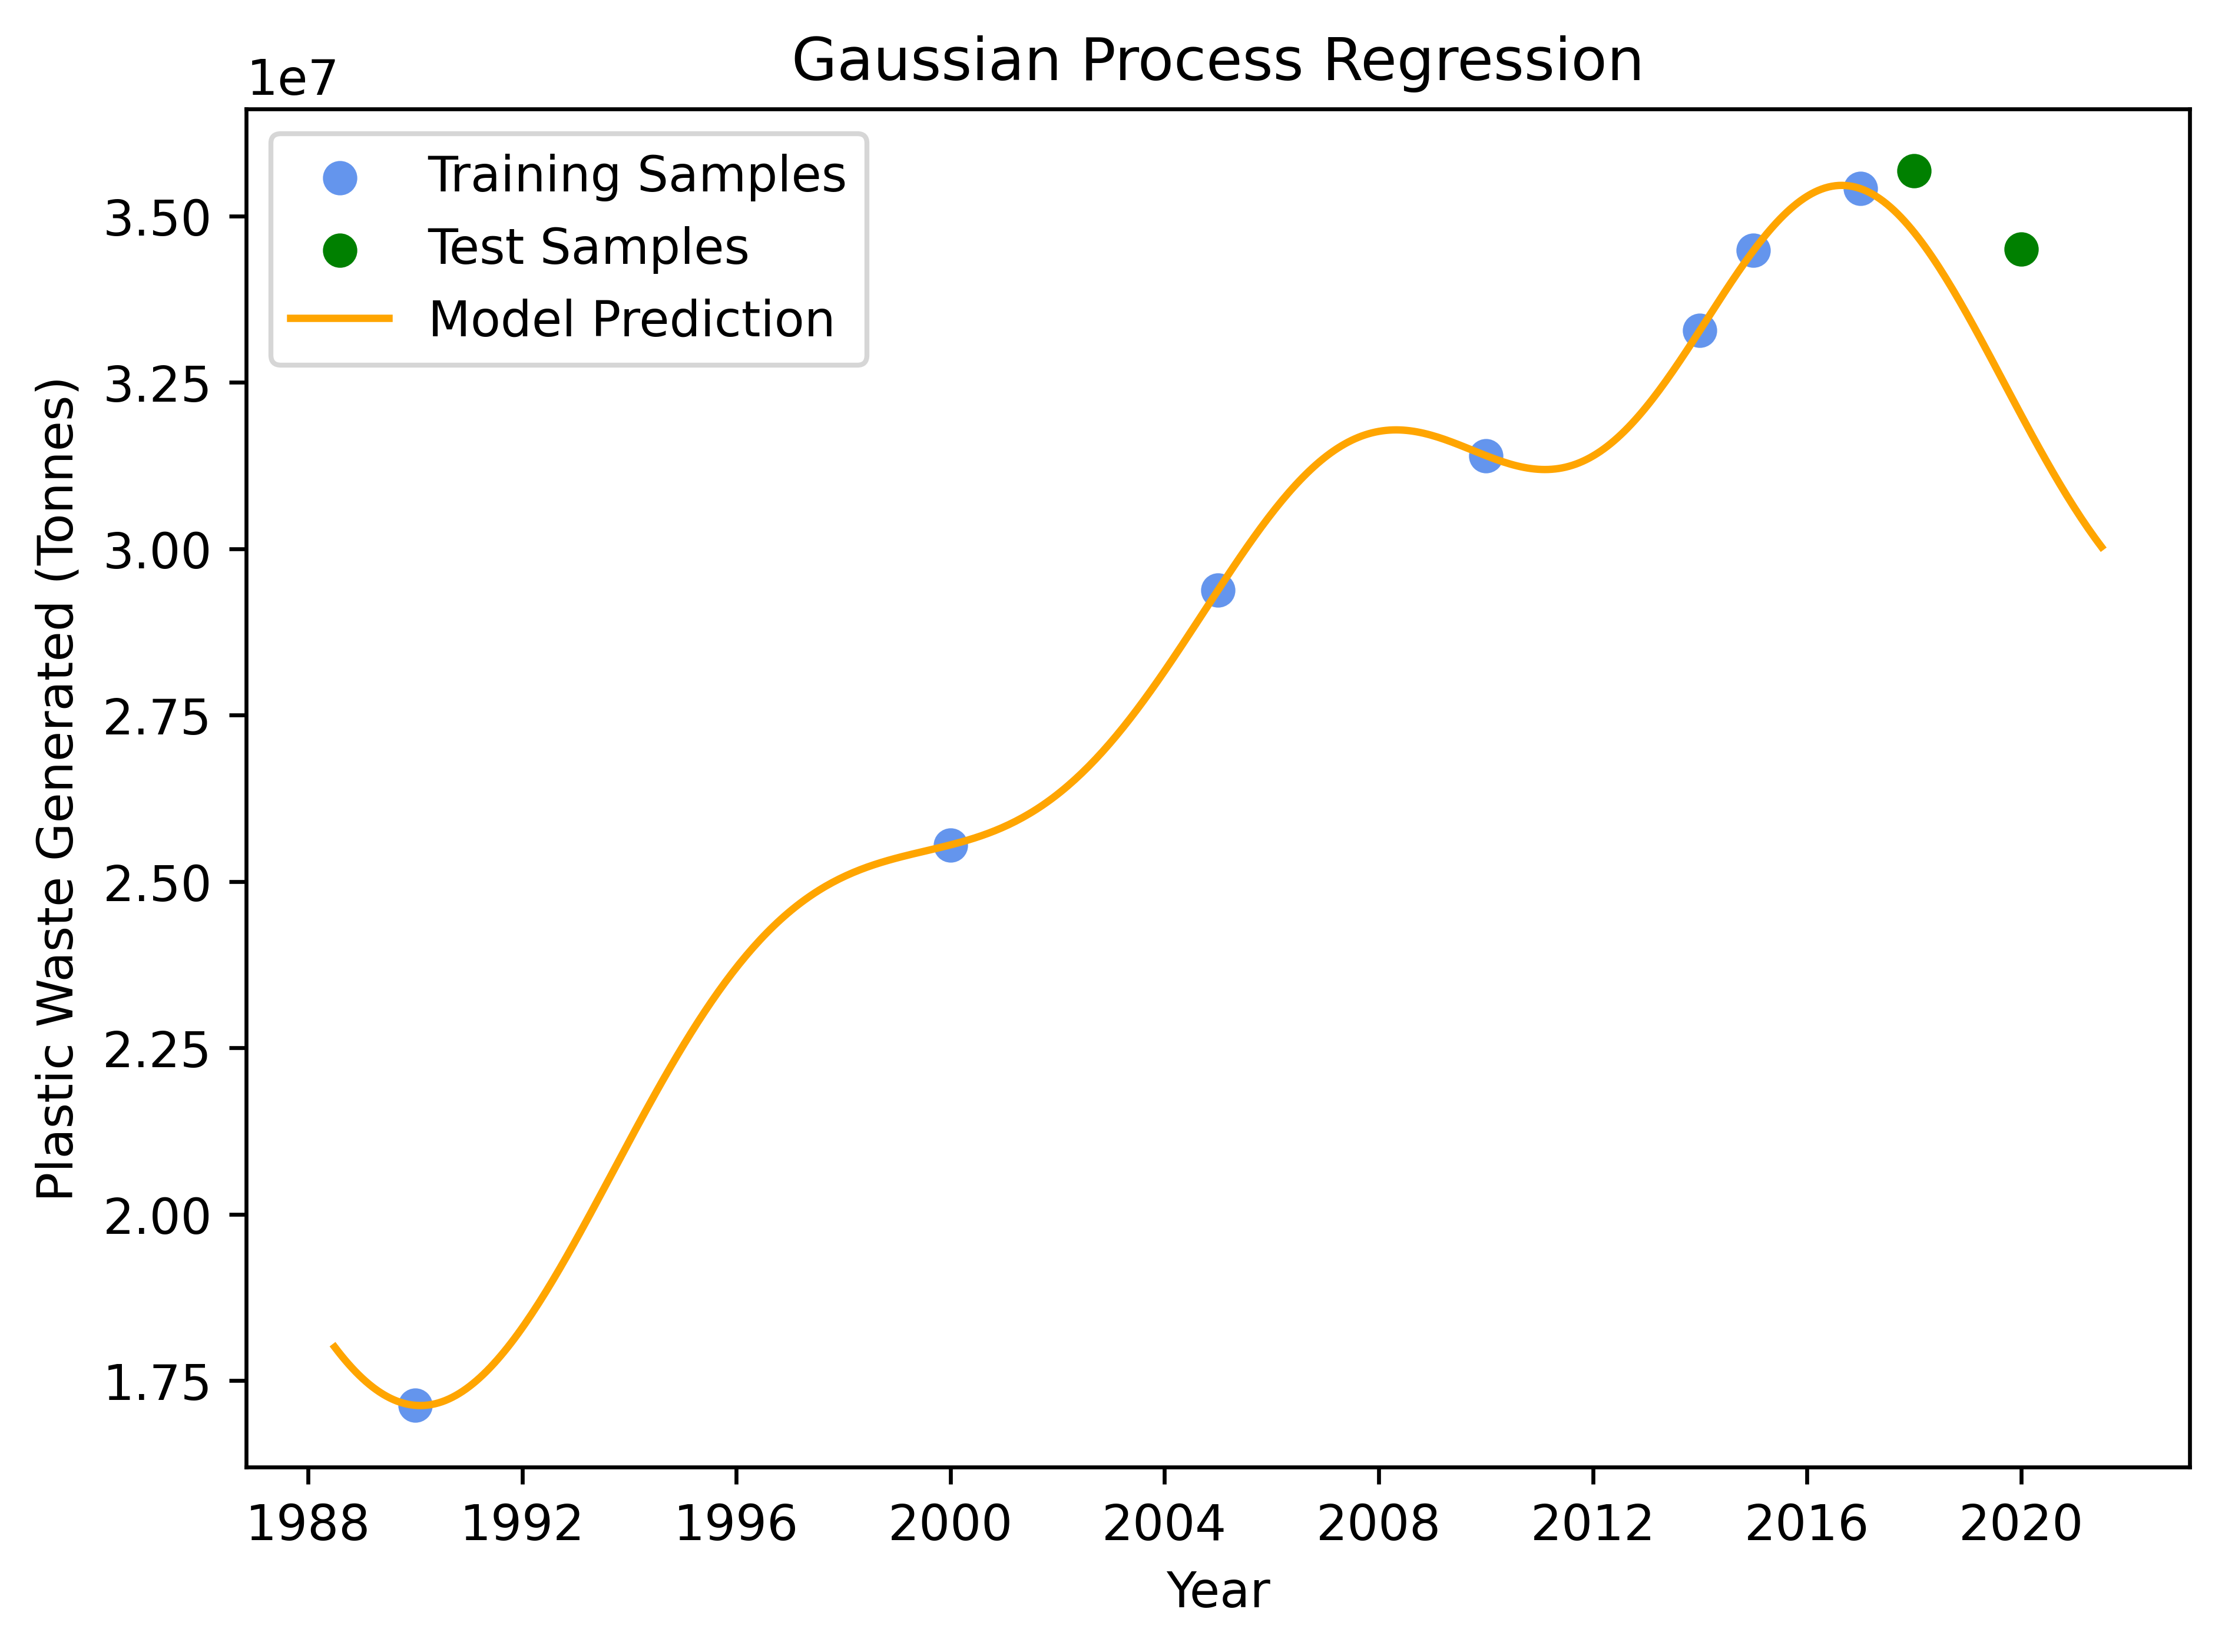
\includegraphics[width=0.45\textwidth]{figures/japan_pwg_forecasting_gpr.png}
	}
	\subfloat[Support vector regression.]{
		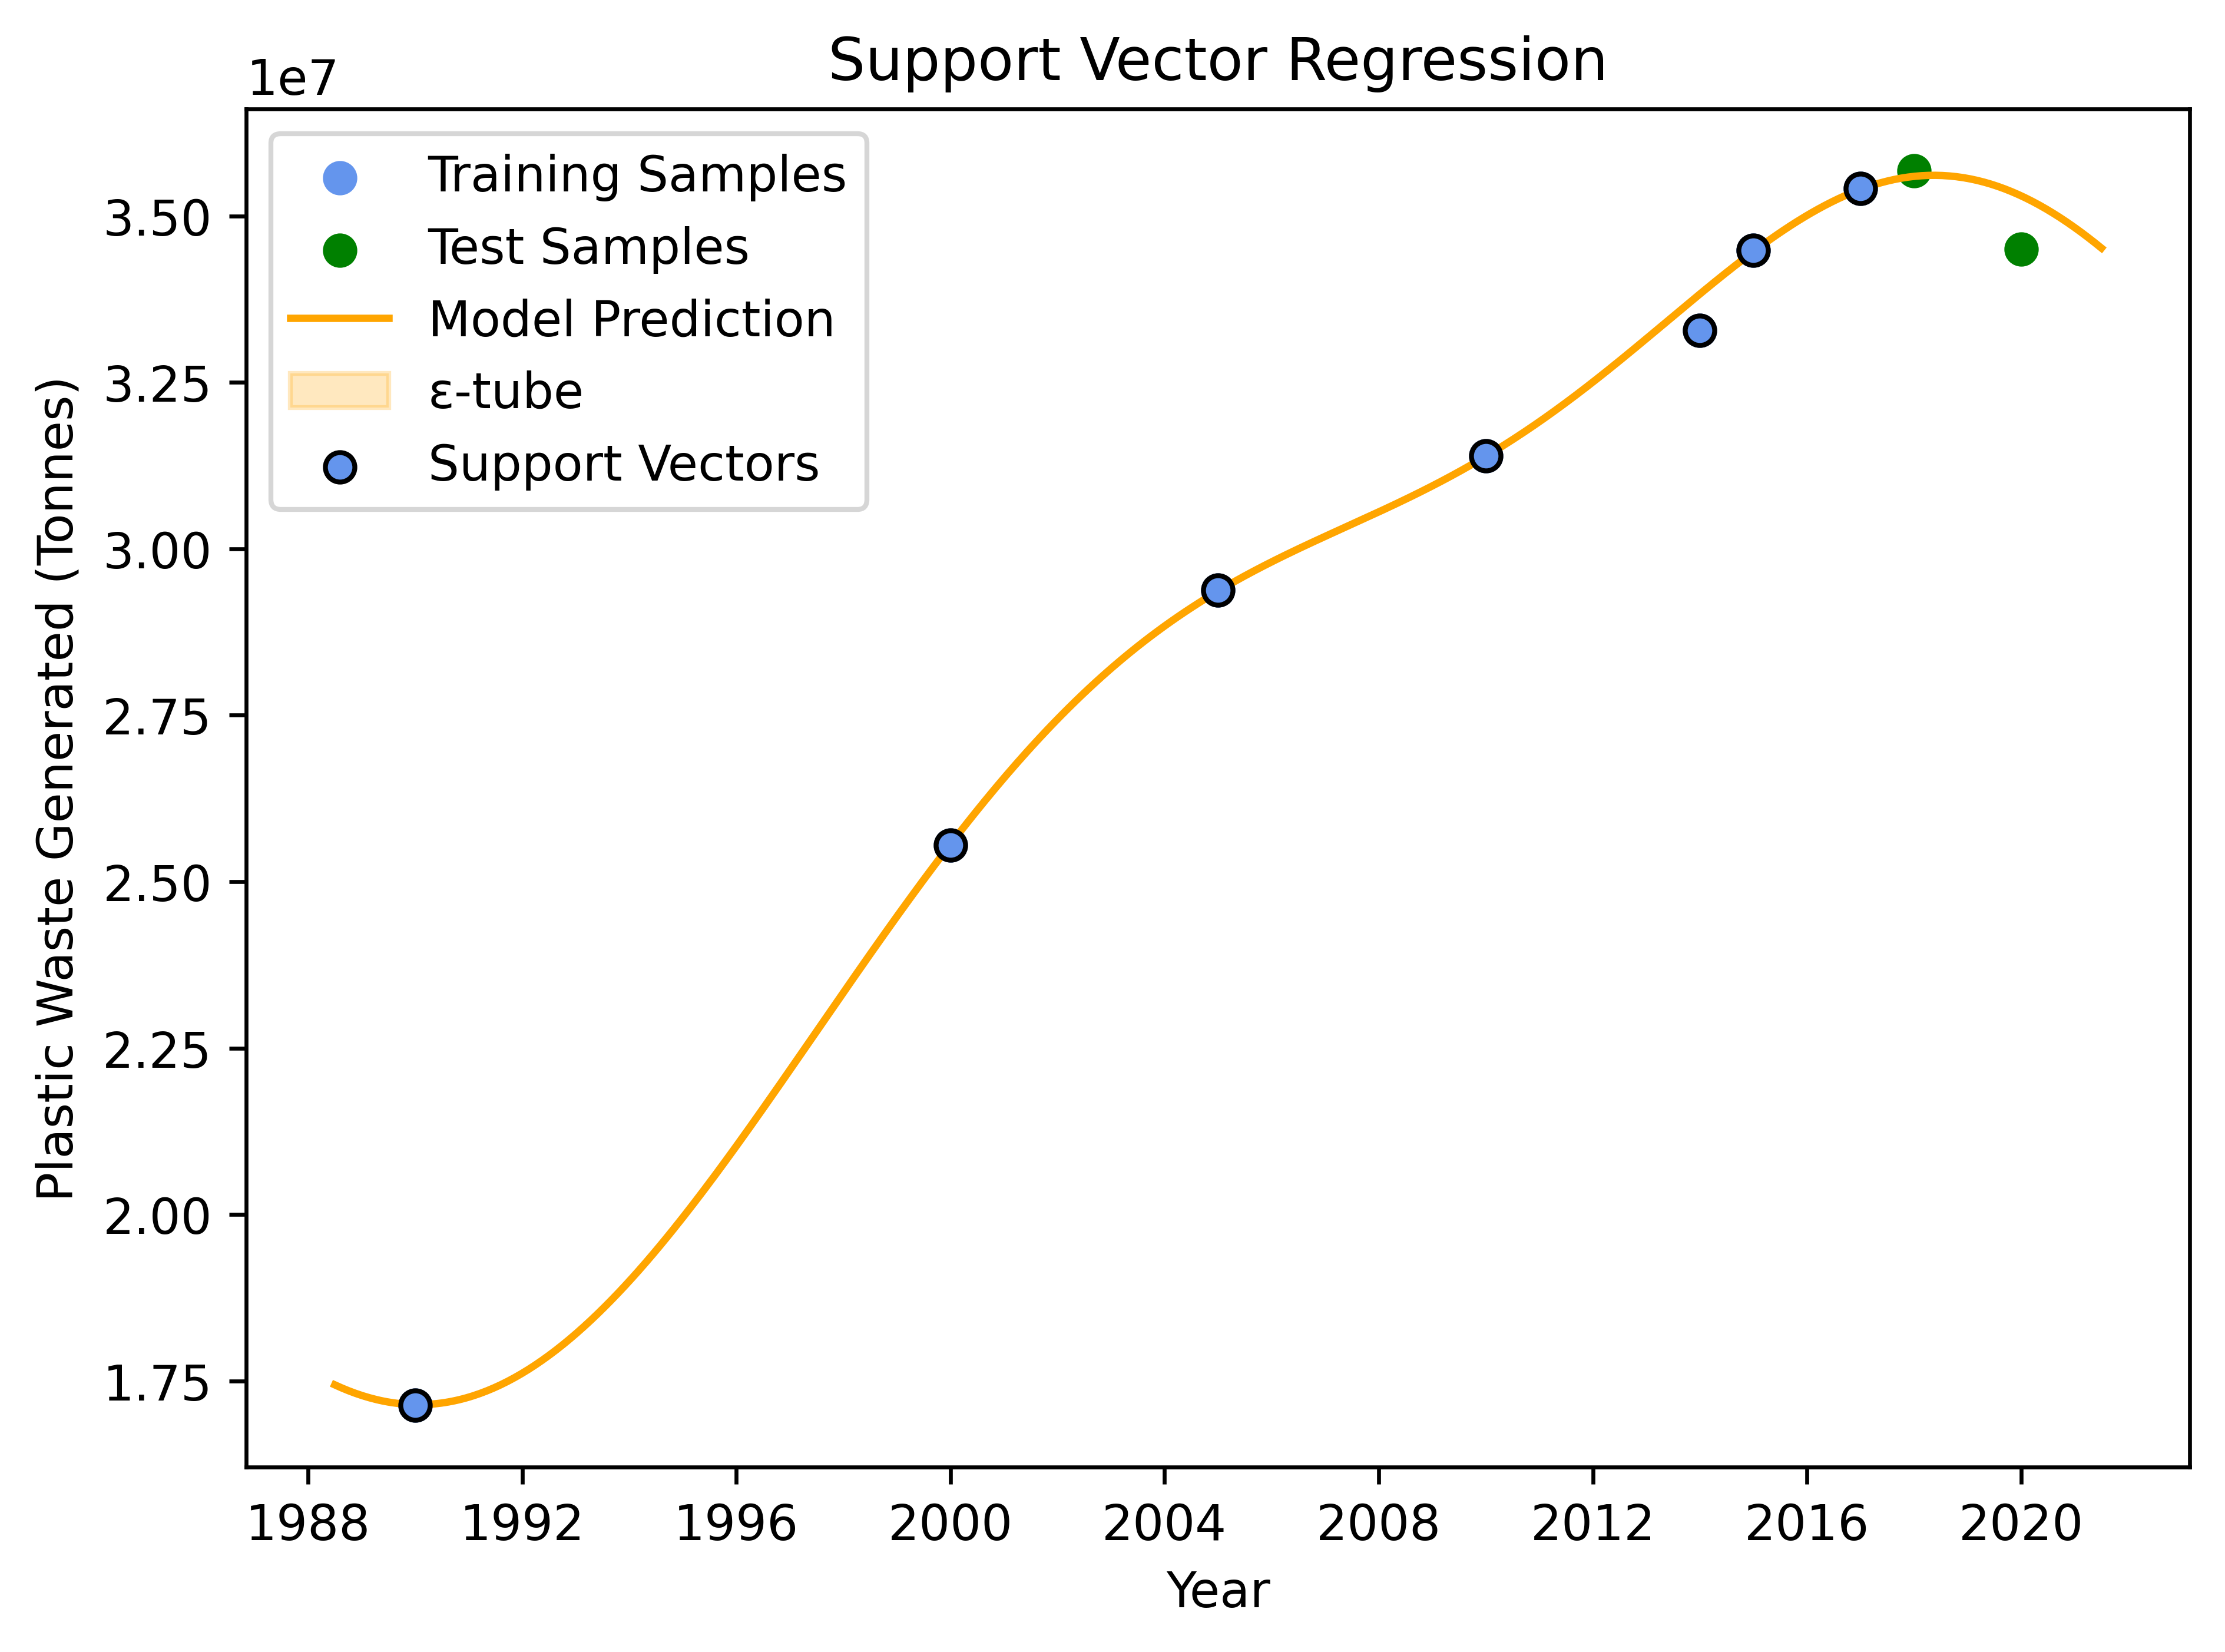
\includegraphics[width=0.45\textwidth]{figures/japan_pwg_forecasting_svr.png}
	}

	\caption{Forecasts of plastic waste generation in Japan by four representative regression models.}
	\label{fig:japan_pwg_forecasting_plots}
\end{figure}

\begin{table}[!ht]
	\centering
	\caption{\centering Temporal forecasting performance for plastic waste generation in Japan using the \texttt{YearPWG (Japan)} dataset.}
	\begin{tabular}{@{}lccccc@{}}
		\toprule
		\textbf{Experiment}                          & \textbf{MAE}          & \textbf{RMSE}         & $\mathbf{R^2}$     & \textbf{WAPE}       & \textbf{MAPE}       \\
		\midrule
		Naive Persistence                            & \(1.800 \times 10^5\) & \(2.110 \times 10^5\) & -0.373             & 4.57\%              & 4.71\%              \\
		Drift Baseline                               & \(1.717 \times 10^5\) & \(1.917 \times 10^5\) & -0.134             & 4.36\%              & 4.47\%              \\
		Exponential Smoothing                        & \(1.379 \times 10^5\) & \(1.424 \times 10^5\) & \(\mathbf{0.374}\) & \(\mathbf{3.50}\)\% & \(\mathbf{3.55}\)\% \\
		Ridge Regression                             & \(5.573 \times 10^5\) & \(5.740 \times 10^5\) & -9.170             & 14.15\%             & 14.33\%             \\
		Gaussian Process Regression                  & \(2.282 \times 10^5\) & \(2.982 \times 10^5\) & -1.745             & 5.79\%              & 6.03\%              \\
		Support Vector Regression                    & \(1.516 \times 10^5\) & \(1.576 \times 10^5\) & 0.234              & 3.85\%              & 3.91\%              \\
		Support Vector Regression\textsuperscript{*} & \(1.452 \times 10^5\) & \(1.839 \times 10^5\) & -0.044             & 3.69\%              & 3.82\%              \\
		Theil-Sen Regression                         & \(1.491 \times 10^5\) & \(2.002 \times 10^5\) & -0.236             & 3.78\%              & 3.95\%              \\
		ARIMA Regression                             & \(2.063 \times 10^5\) & \(2.382 \times 10^5\) & -0.752             & 5.24\%              & 5.39\%              \\
		\hline
	\end{tabular}
	\label{tab:japan_pwg_forecasting_metric_table}
\end{table}

Unlike the global plastics production series, the Japan plastic waste generation series is not monotonic. Figure~\ref{fig:japan_pwg_forecasting_plots} shows that the trend increases in the earlier years, declines sharply, and then partially recovers. This makes the task a useful check of whether flexible regression models can handle short and irregular environmental time series.


Table~\ref{tab:japan_pwg_forecasting_metric_table} shows that exponential smoothing performs best across all reported metrics, with an MAE of \(1.379 \times 10^5\), an RMSE of \(1.424 \times 10^5\), an \(R^2\) of 0.374, a WAPE of 3.50\%, and a MAPE of 3.55\%. The SVR variants and Theil--Sen regression produce competitive percentage errors, but they do not outperform exponential smoothing on the main metrics. Ridge regression performs especially poorly, suggesting that a polynomial trend fitted to this short series is too rigid or unstable for the observed trajectory.

The differences in model performance between the global plastics production and Japan plastic waste generation series suggests that model choice depends strongly on both sample size and trend shape. Flexible machine learning models can perform well when the temporal signal is smooth and enough observations are available, while simple time-series baselines may be more robust for short, non-monotonic country-level series. Combining the data from Experiments 4 and 5, we found that SVR performed generally the best in both experiments.

% ---- Experiment 6: PWDrivers (NN Forecasting)

In Experiment 6, we apply a multilayer perceptron (MLP) model to the \texttt{PWDrivers} dataset. We observe that environmental data in this study is influenced by policy factors, although the dataset does not explicitly include policy-related variables. Therefore, we employ a neural network to capture the implicit relationships between the input features and the target variable, namely plastic waste generation. This experiment evaluates whether the MLP can effectively learn these latent relationships and produce accurate forecasts.

In Experiment 6, we evaluate an MLP model on the pooled \texttt{PWDrivers} dataset. Unlike Experiments 4 and 5, which use year as the only predictor, this experiment uses multiple driver variables, including year, rural population, and urban population. The goal is to test whether a neural network can learn broader cross-country relationships from the pooled driver dataset.

\begin{table}[!ht]
	\centering
	\caption{\centering Neural-network forecasting performance for plastic waste generation on the \texttt{PWDrivers} dataset.}
	\begin{tabular}{@{}lccccc@{}}
		\toprule
		\textbf{Experiment} & \textbf{MAE}           & \textbf{RMSE}          & $\mathbf{R^2}$ & \textbf{WAPE} & \textbf{MAPE} \\
		\midrule
		NN Forecasting      & \(1.401 \times 10^11\) & \(3.158 \times 10^11\) & 0.984          & 24.87\%       & 95.26\%       \\
		\hline
	\end{tabular}
	\label{tab:nn_forecasting_metric_table}
\end{table}

Table~\ref{tab:nn_forecasting_metric_table} shows that the MLP achieves a high \(R^2\) value of 0.984, indicating that it captures much of the overall variance in the test set. However, the percentage-based metrics are much
weaker: WAPE is 24.87\% and MAPE is 95.26\%. This gap suggests that the model fits the large-scale variation in the pooled data, but its relative errors remain substantial for some observations. In other words, the high
\(R^2\) should not be interpreted alone as evidence of uniformly accurate forecasting.

These results show both the potential and the limitation of pooled neural-network forecasting in this setting. The MLP can learn broad patterns from a larger dataset, but the high percentage errors suggest that the pooled
observations are heterogeneous and that the model may struggle with smaller-scale or country-specific behavior. Therefore, Experiment 6 should be viewed as an initial driver-based forecasting benchmark rather than a
definitive forecasting model.

% ---- Experiment 7: PWDrivers (Japan & Slovenia); Multivariate Forecasting

In Experiment 7, we conduct multivariate forecasting using Gaussian Process Regression (GPR), Support Vector Regression (SVR), and MLP models on the \texttt{PWDrivers (Japan)} and \texttt{PWDrivers (Slovenia)} datasets. The MLP model is first pre-trained on the full \texttt{PWDrivers} dataset excluding the target country, and subsequently fine-tuned on the target country's training data. This experiment compares the performance of traditional machine learning methods with that of the MLP in a multivariate forecasting setting. For the \texttt{PWDrivers (Slovenia)} dataset, which contains only \(6\) samples, hyperparameter tuning is not performed due to the limited data availability.

\begin{table}[!ht]
	\centering
	\caption{\centering Multivariate forecasting performance for plastic waste generation in Japan using the \texttt{PWDrivers (Japan)} dataset.}
	\begin{tabular}{@{}lccccc@{}}
		\toprule
		\textbf{Experiment}         & \textbf{MAE}                      & \textbf{RMSE}                     & $\mathbf{R^2}$     & \textbf{WAPE}       & \textbf{MAPE}       \\
		\midrule
		NN Forecasting              & \(\mathbf{4.316 \times 10^{11}}\) & \(\mathbf{4.818 \times 10^{11}}\) & \(\mathbf{0.433}\) & \(\mathbf{7.76}\)\% & 7.42\%              \\
		Support Vector Regression   & \(4.339 \times 10^{11}\)          & \(5.260 \times 10^{11}\)          & 0.324              & 7.80\%              & \(\mathbf{7.29}\)\% \\
		Gaussian Process Regression & \(6.400 \times 10^{11}\)          & \(7.628 \times 10^{11}\)          & -0.420             & 11.51\%             & 10.79\%             \\
		\hline
	\end{tabular}
	\label{tab:multivariate_forecasting_japan_metric_table}
\end{table}

\begin{table}[!ht]
	\centering
	\caption{\centering Multivariate forecasting performance for plastic waste generation in Slovenia using the \texttt{PWDrivers (Slovenia)} dataset.}
	\begin{tabular}{@{}lccccc@{}}
		\toprule
		\textbf{Experiment}         & \textbf{MAE}                   & \textbf{RMSE}                  & $\mathbf{R^2}$      & \textbf{WAPE}       & \textbf{MAPE}       \\
		\midrule
		NN Forecasting              & \(\mathbf{4.235 \times 10^9}\) & \(\mathbf{4.887 \times 10^9}\) & \(\mathbf{-0.075}\) & \(\mathbf{8.56}\)\% & 9.12\%              \\
		Support Vector Regression   & \(4.667 \times 10^9\)          & \(5.146 \times 10^9\)          & -0.192              & 9.44\%              & \(\mathbf{9.10}\)\% \\
		Gaussian Process Regression & \(4.712 \times 10^9\)          & \(5.338 \times 10^9\)          & -0.283              & 9.53\%              & 9.13\%              \\
		\hline
	\end{tabular}
	\label{tab:multivariate_forecasting_slovenia_metric_table}
\end{table}
